\documentclass[11,]{article}
\usepackage{lmodern}
\usepackage{amssymb,amsmath}
\usepackage{ifxetex,ifluatex}
\usepackage{fixltx2e} % provides \textsubscript
\ifnum 0\ifxetex 1\fi\ifluatex 1\fi=0 % if pdftex
  \usepackage[T1]{fontenc}
  \usepackage[utf8]{inputenc}
\else % if luatex or xelatex
  \ifxetex
    \usepackage{mathspec}
  \else
    \usepackage{fontspec}
  \fi
  \defaultfontfeatures{Ligatures=TeX,Scale=MatchLowercase}
\fi
% use upquote if available, for straight quotes in verbatim environments
\IfFileExists{upquote.sty}{\usepackage{upquote}}{}
% use microtype if available
\IfFileExists{microtype.sty}{%
\usepackage{microtype}
\UseMicrotypeSet[protrusion]{basicmath} % disable protrusion for tt fonts
}{}
\usepackage[margin=1in]{geometry}
\usepackage{hyperref}
\hypersetup{unicode=true,
            pdftitle={The information content of StockTwits},
            pdfauthor={Joyce Cahoon},
            pdfborder={0 0 0},
            breaklinks=true}
\urlstyle{same}  % don't use monospace font for urls
\usepackage{color}
\usepackage{fancyvrb}
\newcommand{\VerbBar}{|}
\newcommand{\VERB}{\Verb[commandchars=\\\{\}]}
\DefineVerbatimEnvironment{Highlighting}{Verbatim}{commandchars=\\\{\}}
% Add ',fontsize=\small' for more characters per line
\usepackage{framed}
\definecolor{shadecolor}{RGB}{248,248,248}
\newenvironment{Shaded}{\begin{snugshade}}{\end{snugshade}}
\newcommand{\AlertTok}[1]{\textcolor[rgb]{0.94,0.16,0.16}{#1}}
\newcommand{\AnnotationTok}[1]{\textcolor[rgb]{0.56,0.35,0.01}{\textbf{\textit{#1}}}}
\newcommand{\AttributeTok}[1]{\textcolor[rgb]{0.77,0.63,0.00}{#1}}
\newcommand{\BaseNTok}[1]{\textcolor[rgb]{0.00,0.00,0.81}{#1}}
\newcommand{\BuiltInTok}[1]{#1}
\newcommand{\CharTok}[1]{\textcolor[rgb]{0.31,0.60,0.02}{#1}}
\newcommand{\CommentTok}[1]{\textcolor[rgb]{0.56,0.35,0.01}{\textit{#1}}}
\newcommand{\CommentVarTok}[1]{\textcolor[rgb]{0.56,0.35,0.01}{\textbf{\textit{#1}}}}
\newcommand{\ConstantTok}[1]{\textcolor[rgb]{0.00,0.00,0.00}{#1}}
\newcommand{\ControlFlowTok}[1]{\textcolor[rgb]{0.13,0.29,0.53}{\textbf{#1}}}
\newcommand{\DataTypeTok}[1]{\textcolor[rgb]{0.13,0.29,0.53}{#1}}
\newcommand{\DecValTok}[1]{\textcolor[rgb]{0.00,0.00,0.81}{#1}}
\newcommand{\DocumentationTok}[1]{\textcolor[rgb]{0.56,0.35,0.01}{\textbf{\textit{#1}}}}
\newcommand{\ErrorTok}[1]{\textcolor[rgb]{0.64,0.00,0.00}{\textbf{#1}}}
\newcommand{\ExtensionTok}[1]{#1}
\newcommand{\FloatTok}[1]{\textcolor[rgb]{0.00,0.00,0.81}{#1}}
\newcommand{\FunctionTok}[1]{\textcolor[rgb]{0.00,0.00,0.00}{#1}}
\newcommand{\ImportTok}[1]{#1}
\newcommand{\InformationTok}[1]{\textcolor[rgb]{0.56,0.35,0.01}{\textbf{\textit{#1}}}}
\newcommand{\KeywordTok}[1]{\textcolor[rgb]{0.13,0.29,0.53}{\textbf{#1}}}
\newcommand{\NormalTok}[1]{#1}
\newcommand{\OperatorTok}[1]{\textcolor[rgb]{0.81,0.36,0.00}{\textbf{#1}}}
\newcommand{\OtherTok}[1]{\textcolor[rgb]{0.56,0.35,0.01}{#1}}
\newcommand{\PreprocessorTok}[1]{\textcolor[rgb]{0.56,0.35,0.01}{\textit{#1}}}
\newcommand{\RegionMarkerTok}[1]{#1}
\newcommand{\SpecialCharTok}[1]{\textcolor[rgb]{0.00,0.00,0.00}{#1}}
\newcommand{\SpecialStringTok}[1]{\textcolor[rgb]{0.31,0.60,0.02}{#1}}
\newcommand{\StringTok}[1]{\textcolor[rgb]{0.31,0.60,0.02}{#1}}
\newcommand{\VariableTok}[1]{\textcolor[rgb]{0.00,0.00,0.00}{#1}}
\newcommand{\VerbatimStringTok}[1]{\textcolor[rgb]{0.31,0.60,0.02}{#1}}
\newcommand{\WarningTok}[1]{\textcolor[rgb]{0.56,0.35,0.01}{\textbf{\textit{#1}}}}
\usepackage{graphicx,grffile}
\makeatletter
\def\maxwidth{\ifdim\Gin@nat@width>\linewidth\linewidth\else\Gin@nat@width\fi}
\def\maxheight{\ifdim\Gin@nat@height>\textheight\textheight\else\Gin@nat@height\fi}
\makeatother
% Scale images if necessary, so that they will not overflow the page
% margins by default, and it is still possible to overwrite the defaults
% using explicit options in \includegraphics[width, height, ...]{}
\setkeys{Gin}{width=\maxwidth,height=\maxheight,keepaspectratio}
\IfFileExists{parskip.sty}{%
\usepackage{parskip}
}{% else
\setlength{\parindent}{0pt}
\setlength{\parskip}{6pt plus 2pt minus 1pt}
}
\setlength{\emergencystretch}{3em}  % prevent overfull lines
\providecommand{\tightlist}{%
  \setlength{\itemsep}{0pt}\setlength{\parskip}{0pt}}
\setcounter{secnumdepth}{0}
% Redefines (sub)paragraphs to behave more like sections
\ifx\paragraph\undefined\else
\let\oldparagraph\paragraph
\renewcommand{\paragraph}[1]{\oldparagraph{#1}\mbox{}}
\fi
\ifx\subparagraph\undefined\else
\let\oldsubparagraph\subparagraph
\renewcommand{\subparagraph}[1]{\oldsubparagraph{#1}\mbox{}}
\fi

%%% Use protect on footnotes to avoid problems with footnotes in titles
\let\rmarkdownfootnote\footnote%
\def\footnote{\protect\rmarkdownfootnote}

%%% Change title format to be more compact
\usepackage{titling}

% Create subtitle command for use in maketitle
\newcommand{\subtitle}[1]{
  \posttitle{
    \begin{center}\large#1\end{center}
    }
}

\setlength{\droptitle}{-2em}

  \title{The information content of StockTwits}
    \pretitle{\vspace{\droptitle}\centering\huge}
  \posttitle{\par}
    \author{Joyce Cahoon}
    \preauthor{\centering\large\emph}
  \postauthor{\par}
    \date{}
    \predate{}\postdate{}
  
\usepackage{placeins}
\usepackage{chngcntr}
\usepackage{multicol}
\usepackage{setspace}
\usepackage{mathrsfs}
\usepackage{amsthm}
\usepackage{graphicx}
\usepackage{booktabs}
\usepackage{multirow}
\usepackage{subcaption}
\usepackage{sidecap}
\usepackage{mathtools}
\usepackage{bm}
\usepackage[linesnumbered,algoruled,boxed,lined,commentsnumbered]{algorithm2e}
\SetKwInput{KwInput}{Input}
\SetKwInput{KwOutput}{Output}
\onehalfspacing
\setlength{\parskip}{8.0pt}
\newcommand{\V}[1]{{\bm{#1}}}
\newcommand{\Real}{\mathbb{R}}
\newcommand{\Exp}{\mathbb{E}}
\newcommand{\ubar}[1]{\underbar{$#1$}}
\newcommand{\obar}{\overline}
\newtheorem{walley781}{Theorem}
\usepackage[symbols,nogroupskip,nonumberlist,automake]{glossaries-extra}
\makeglossaries
\newglossaryentry{T}{name=\ensuremath{T}, description={Number of topics},type=symbols}

\begin{document}
\maketitle
\begin{abstract}
blah
\end{abstract}

{
\setcounter{tocdepth}{2}
\tableofcontents
}
\newpage

\hypertarget{introduction}{%
\section{Introduction}\label{introduction}}

As fund managers, we were tasked with constructing a cross-sectional,
long-short US equity strategy on
\href{https://www.quantopian.com/}{Quantopian}. There were not many
explicit constraints on the specific strategy we utilized, but it must
pass the following criteria: (i) trade liquid stocks, (ii) have no more
than 5\% of capital invested in any one asset, (iii) have no more than
10\% net dollar exposure, (iv) achieve mean daily turnover between 5\%
and 65\% over a 63-trading-day rolling window, (v) attain gross leverage
between 0.8x and 1.1x, (vi) have low correlation to the market, (vii)
have less than 20\% exposed to each of the 11 sectors as defined on
Quantopian, and (viii) result in positive returns. While the last return
criteria was not a constraint we included in our optimization, we did
design our algorithm with the rest of the seven criteria in mind
(Quantopian \protect\hyperlink{ref-q}{2018}).

The algorithm I eventually submitted was one based purely on the
information content from StockTwits; more specifically, the 5-day moving
average of the bull minus bear intensity associated with each tradable
stock. I rely on this metric to assign each stock's weight in our
portfolio, subject to certain constraints so that our algorithm passes
\texttt{Quantopian}'s criteria to remain in competition. Given the large
literature around news and social media sentiment in driving volatility
and liquidity in the market, I wanted to examine the power of this
unstructured data in driving returns.

My algorithm's performance over the November period resulted in a final
rank of 105 out of 261 submissions and a total score of 0.338. Its
performance is mediocre at best and can be attributed the fact that the
tuning mechanism for my input parameters was based only on the backtest
returns. Given the constraints and the length of moving window for our
sentiment metric was overfit to a backtest window between 2016 and 2018,
my strategy may have experienced bad out-of-sample performance.

Nevertheless, this strategy did perform within the top 40\% of all
submissions, which corroborates many findings in literature that social
media has some effect on driving prices. The majority of literature
suggests extreme sentiment or extreme volume of online media content
tends to drive the positive and negative returns, and since the month of
November can be characterized by extreme volatility this may explain the
high performance of our sentiment strategy. As expected, for December,
the peaks in the VIX, however, have subsided given greater clarity
around the Trump administration's trade policy and Fed's decision to
stop raising rates, and our strategy fell a few ranks to 113 with a
score of 0.316 (Gurdus \protect\hyperlink{ref-cramer2018}{2018}).

\hypertarget{related-work}{%
\section{Related Work}\label{related-work}}

The first paper that explored the relationship of text---unstructured
data---in driving stock prices was Cutler et al.
(\protect\hyperlink{ref-cutler1988}{1988})'s ``What moves stock
prices?'' At the time, the field of computational linguistics was yet
sophisticated enough to process large collections of text, so Cutler and
his team examined 49 major events discussed in the NY Times Business
desk and assessed the market changes associated with each event.
Unfortunately, given the number of significant market moves associated
with days where nothing significant was released, they were unable to
identify any link between market moves and news, possibly stymeing
explorations into this realm (Cutler et al.
\protect\hyperlink{ref-cutler1988}{1988}). Fortunately, another
empirical study emerged in 1998, which leveraged information on online
message boards instead, identifying strong correlations between stocks
with high message volume and high market valuation. In fact, Wysocki
found message volume forecasted not only abnormal stock returns the next
day, but also trading volume the next day (Wysocki
\protect\hyperlink{ref-wysocki1998}{1998}).

Yet, given these results and similar findings from papers like Bagnoli
et al. (\protect\hyperlink{ref-bagnoli1999}{1999}), Antweiler and Frank
(\protect\hyperlink{ref-antweiler2004}{2004}), corroborating the link
between prices and social chatter, a number of studies find the
opposite. Tumarkin and Whitelaw
(\protect\hyperlink{ref-tumarkin2001}{2001}) found no relationship for
equities in the tech sector and the message activity on RagingBull.com.
Das and Chen (\protect\hyperlink{ref-das2007}{2007}) developed a
classifier for investor sentiment from message board text, yet were
unable to to demonstrate its ability to forecast returns. Dewally
(\protect\hyperlink{ref-dewally2003}{2003}) found recommendations
exchanged on sites like \texttt{misc.invest.stocks} and
\texttt{alt.invest.penny-stocks} had no effect on the return
characteristics of the stocks under discussion.

Despite these mixed claims, newer studies arose reporting the opposite.
In fact, the seminar paper by Tetlock
(\protect\hyperlink{ref-tetlock2007}{2007}) concluded high negative
sentiment in the Wall Street Journal predicted temporary downward price
pressure, echoing the thoughts expressed in Wysocki
(\protect\hyperlink{ref-wysocki1998}{1998}) that extreme news affects
market movement. Additional works that build on Tetlock's use of news as
a fundamental factor is Mitra et al.
(\protect\hyperlink{ref-mitra2008}{2008}), Leinweber and Sisk
(\protect\hyperlink{ref-leinweber2011}{2011}) and Fang and Peress
(\protect\hyperlink{ref-fang2009}{2009}), each providing evidence for
the predictive value in social chatter. In this class, we were also
directed to the paper by Agrawal et al.
(\protect\hyperlink{ref-agrawal2019}{2019}), which provides a great
overview of literature that further promotes the use of Twitter and
StockTwits to predict stock volatility, liquidity and return.

\hypertarget{our-reliance-on-stocktwits}{%
\section{Our Reliance on StockTwits}\label{our-reliance-on-stocktwits}}

Key to my strategy is the output from the \texttt{bull\_minus\_bear} API
call as it is this signal that is fed into the optimization function and
this result that determines the order size of each asset. While there is
no disclosure on the natural language processing model that calculates
the bull and bear intensity of each social media message, it is helpful
to look at examples and understand the nature of posts that ultimately
determine the power of our sentiment measure.

\begin{figure}

{\centering 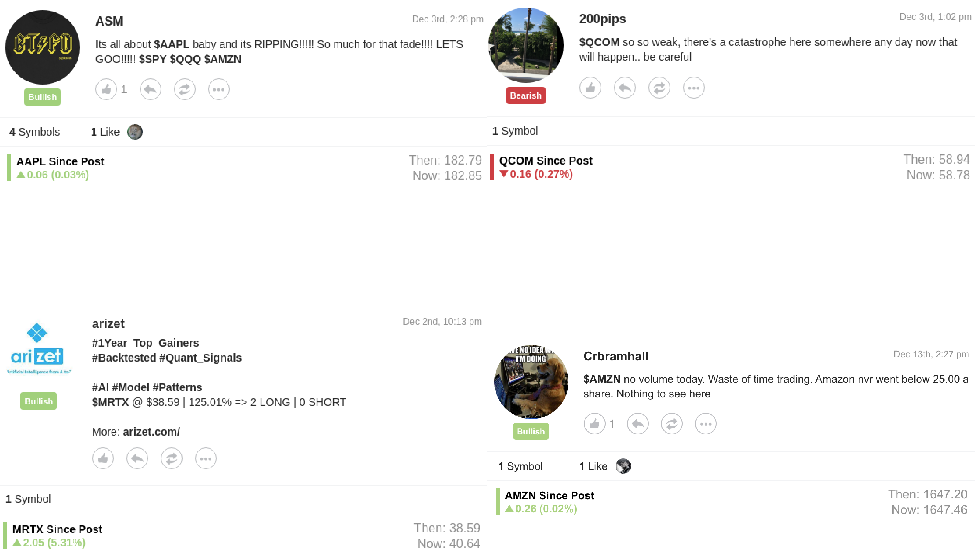
\includegraphics[width=0.8\linewidth]{cahoon_final_paper_files/figure-latex/unnamed-chunk-2-1} 

}

\caption{\label{StockT}Four examples of messages posted on StockTwits. The bull and bear indicator is provided by the user, and all stock tickers that follow the cashtag is associated with this indicator. The bull and bear intensity is then computed by a proprietary StockTwits algorithm based on the content within each individual post.}\label{fig:unnamed-chunk-2}
\end{figure}

As shown in Figure \ref{StockT}, there is a lot of noise in StockTwit
data as users each utilize the platform for different reasons and do not
have to disclose any of their personal stakes in the equities they
support. Logically, users that are more influential should have a higher
impact in driving overall investor sentiment, and thus driving prices,
but there currently is no easily available API call that provides such a
weighting. Moreover, these influencers change over time, increasing the
difficulty around identifying posts that might contain more information
than another. As a result, relying on the aggregate bullish and bearish
intensity averaged daily across all the tagged StockTwits messages is
the best surrogate we have to understanding community sentiment over a
specific stock.

From the free version of StockTwits API, we have access to the following
daily metrics for 10,214 liquid US equities:

\begin{itemize}
\tightlist
\item
  \emph{Bull and bear scored messages}: Total number of daily messages
  that were labeled either ``Bullish'' or ``Bearish'' on the StockTwits
  platform by the user
\item
  \emph{Bull or bear intensity}: Daily score between 0 and 4 aggregated
  across processed messages. 0 means no bull or bear sentiment was
  detected by StockTwits proprietary trading algorithm. 4 means very
  high bull or bear sentiment was detected.
\item
  \emph{Total scanned}: Total number of daily messages that appear on
  StockTwits platform that has at least one cashtag associated with it.
  The message is included in this count whether it is labeled or
  unlabeled and can be processed by the StockTwist language algorithm or
  not.
\end{itemize}

Since disagreement among message content has been shown to be associated
with greater liquidity and volatility, we focus on the metric of
\texttt{bull\_minus\_bear} as it is one proxy for disagreement among
investor opinion (Antweiler and Frank
\protect\hyperlink{ref-antweiler2004}{2004}). Given the overall trend in
this metric is not stable as we will see in Figure \ref{tops}, a moving
average is taken. Eventually, I settle on 5-day moving average as the
mean information coefficient (IC) is positive that this point. The IC is
often chosen as a means to evaluate whether a factor is predictive of
returns as it is more robust to outliers and normality assumptions,
allowing one to better tease out whether two series move in concert or
not. It is thus calculated from the rank of each data pair in each
series as \(IC = 1- 6\sum_i d_i^2 / n(n^2-1)\) where \(d_i\) represents
the difference in ranks. As shown in the top left of Figure \ref{IC},
prior to 5 trading days, our sentiment signal hurts our returns in that
its forecast is negative, but after 5 trading days, we gain some
predictive power. This is further corroborated in the top right plot in
that returns are highest when the signal is delayed by four days.

Given the IC results, we may want to build greater exposure to this
factor as it still benefits us after 10 trading days. We can also
leverage the positive effects of this factor by increasing our turnover
constraints as it appears it does not hurt our portfolio to keep in
there for a longer period of time. Another asset is that our sentiment
factor has relatively low exposures throughout, with most of the returns
from volatility risk. However, there does appear to be persistent
exposure to value and short term reversal, in that it is shifted to the
left of zero; and persistent exposure to size and momentum, in that it
is shifted to the right of zero. Ideally, we would choose a factor that
doesn't display this skew, but the skew does not appear too large. We
benefit from the fact that the width of each of our box and whisker
plots are not that wide, so our exposures do not vary much over time.

Unfortunately, when we examine our exposures through cumulative returns
and volatility, we find that our sentiment factor may not be as strong
as we desired. As shown by the left bar graph in Figure \ref{IC}, most
of our returns are obtained from exposure to common risk factors, and,
as shown in the right bar graph, are in fact driven by these common risk
factors. Ideally, we would like to strip away the contribution from
these common risk factors as portfolio performance from this exposure
can easily be replicated from ETFs or other easy, cost-effective
methods. We can also work to identify asset classes to include in our
portfolio that would offset the exposure risks identified above.
Nevertheless, this factor analysis was conducted only over the sentiment
signal in 2018, so there may be other extended periods prior to 2018 in
which our factor over or underperforms.

\begin{figure}

{\centering 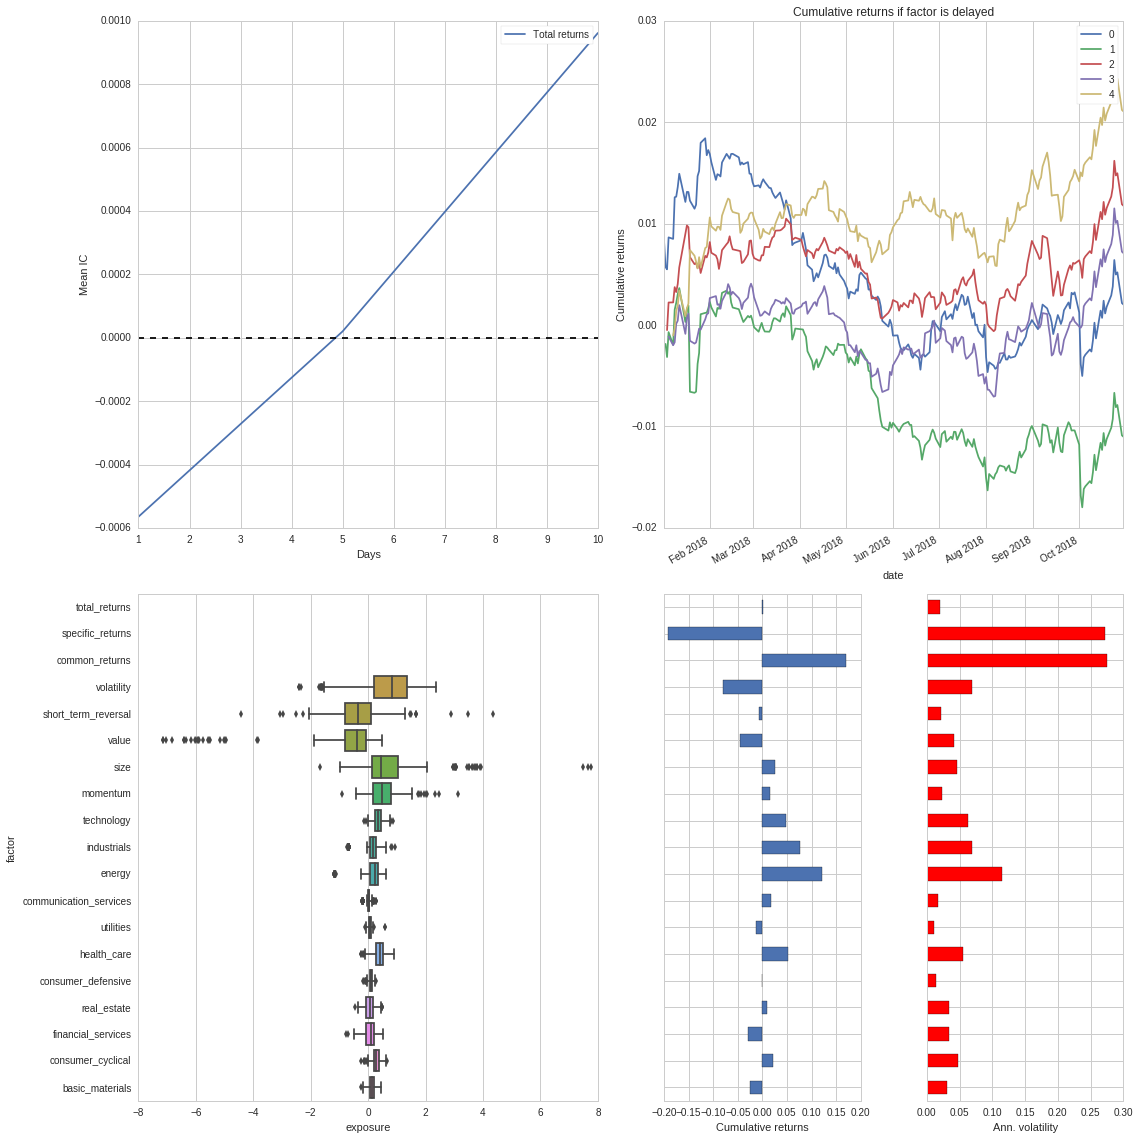
\includegraphics[width=0.8\linewidth]{~/workspace/st790-financial-stats/final/download2} 

}

\caption{\label{IC}Examination of (top-right) information coefficient averaged over all possible asset returns, (top-left) cumulative returns when factor is delayed, (bottom-left) risk exposures, and (bottom-right) cumulative returns and volatility.}\label{fig:unnamed-chunk-3}
\end{figure}

\hypertarget{trading-strategy}{%
\section{Trading Strategy}\label{trading-strategy}}

Given the ease of implementation and some good alpha characteristics as
delineated above, we chose to rely on the sentiment factor in our
trading strategy. Continuous backtesting was run to derive the
constraint parameters as outlined:

\begin{enumerate}
\def\labelenumi{\arabic{enumi}.}
\tightlist
\item
  Once a week, we choose a universe of liquid assets from
  \(\texttt{QTradeableStocksUS}\) that pass the following filters:

  \begin{itemize}
  \tightlist
  \item
    It is not trading within 2 days of any earnings announcements as
    assets are generally more volatile within these dates.
  \item
    It has not been announced as an acquisition target. To further
    reduce any possible volatility, we avoid acquisition targets as they
    often pose huge risk to quant strategies.
  \item
    We are able to calculate a 5 day moving average of the
    bull-minus-bear signal from the \(\texttt{StockTwits}\) API.
  \end{itemize}
\item
  Every day, we build an alpha vector for the universe of liquid assets
  filtered from our step above. The alpha model we use is quite simple:
  we rank the assets by its bull-to-bear intensity, averaged over the
  past 5 days as evaluated from StockTwits, and find a set of new
  portfolio weights that maximizes the sum of each asset's weight times
  this alpha value. Our objective defined in \texttt{MaximizeAlpha} is
  thus simply a function of this sentiment datastream as we believe this
  ranking is similar to expected returns of each asset. As a result, our
  routine effectively goes long on assets with high bullish signal and
  short on those with a high bearish signal.
\item
  Once a week, we calculate the portfolio that maximizes the
  alpha-weighted sum of our position sizes, subject to the following
  constraints:

  \begin{itemize}
  \tightlist
  \item
    Our portfolio maintains a gross leverage of, or less than, 1.0x.
  \item
    Our portfolio has no more than 5\% in any single asset.
  \item
    Our portfolio does not pass mean daily turnover of 80\%.
  \end{itemize}
\end{enumerate}

Our simple strategy can thus be summarized as follows:

\[
\max_{{\bm{w}} \in \mathbb{R}^n} {\bm{\alpha}}^T {\bm{w}} \quad \text{subject to} \quad |w_i| \leq 0.05,\; \sum_i |w_i| \leq  1.00, \; \sum_i |w_i-w_{i-1}| \leq 0.80, \; \sum_i w_i = 1
\] \noindent where \({\bm{w}}\) represents the weights attached to each
asset in our optimal portfolio.

\hypertarget{backtest-analysis}{%
\section{Backtest Analysis}\label{backtest-analysis}}

\hypertarget{performance}{%
\section{Performance}\label{performance}}

we achieve the following leaderboard results at the end of our one-month
trading period from November \(1^{st}\) to November \(30^{th}\):

\hypertarget{discussion}{%
\section{Discussion}\label{discussion}}

Section 7 will be the conclusion and discussion. You may revisit the
advantage and disadvantage of your strategy and provide some insights
for future exploration directions.~ In the appendix, all your programing
codes should be attached.~

\hypertarget{appendix}{%
\section{Appendix}\label{appendix}}

\hypertarget{quantopian-submission}{%
\subsection{Quantopian Submission}\label{quantopian-submission}}

\begin{Shaded}
\begin{Highlighting}[]
\CommentTok{# Import Algorithm API functions}
\ImportTok{from}\NormalTok{ quantopian.algorithm }\ImportTok{import}\NormalTok{ (}
\NormalTok{    attach_pipeline,}
\NormalTok{    pipeline_output,}
\NormalTok{    order_optimal_portfolio,}
\NormalTok{)}
\CommentTok{# Import Optimize API module}
\ImportTok{import}\NormalTok{ quantopian.optimize }\ImportTok{as}\NormalTok{ opt}
\CommentTok{# Pipeline imports}
\ImportTok{from}\NormalTok{ quantopian.pipeline }\ImportTok{import}\NormalTok{ Pipeline}
\ImportTok{from}\NormalTok{ quantopian.pipeline.data.psychsignal }\ImportTok{import}\NormalTok{ stocktwits}
\ImportTok{from}\NormalTok{ quantopian.pipeline.factors }\ImportTok{import}\NormalTok{ SimpleMovingAverage}
\CommentTok{# Import built-in universe and Risk API method}
\ImportTok{from}\NormalTok{ quantopian.pipeline.filters }\ImportTok{import}\NormalTok{ QTradableStocksUS}
\ImportTok{from}\NormalTok{ quantopian.pipeline.experimental }\ImportTok{import}\NormalTok{ risk_loading_pipeline}
\CommentTok{# Get event data }
\ImportTok{from}\NormalTok{ quantopian.pipeline.factors.eventvestor }\ImportTok{import}\NormalTok{ (}
\NormalTok{    BusinessDaysUntilNextEarnings,}
\NormalTok{    BusinessDaysSincePreviousEarnings,}
\NormalTok{)}
\ImportTok{from}\NormalTok{ quantopian.pipeline.filters.eventvestor }\ImportTok{import}\NormalTok{ IsAnnouncedAcqTarget}
\ImportTok{from}\NormalTok{ quantopian.pipeline.factors }\ImportTok{import}\NormalTok{ BusinessDaysSincePreviousEvent}
\KeywordTok{def}\NormalTok{ initialize(context):}
    \CommentTok{# Constraint parameters}
\NormalTok{    context.max_leverage }\OperatorTok{=} \FloatTok{1.0}
\NormalTok{    context.max_pos_size }\OperatorTok{=} \FloatTok{0.05}
\NormalTok{    context.max_turnover }\OperatorTok{=} \FloatTok{0.8}
    \CommentTok{# Attach data pipelines}
\NormalTok{    attach_pipeline(}
\NormalTok{        make_pipeline(),}
        \StringTok{'data_pipe'}
\NormalTok{    )}
\NormalTok{    attach_pipeline(}
\NormalTok{        risk_loading_pipeline(),}
        \StringTok{'risk_pipe'}
\NormalTok{    )}
    \CommentTok{# Schedule rebalance function}
\NormalTok{    schedule_function(}
\NormalTok{        rebalance,}
\NormalTok{        date_rules.week_start(),}
\NormalTok{        time_rules.market_open(),}
\NormalTok{    )}
\KeywordTok{def}\NormalTok{ before_trading_start(context, data):}
    \CommentTok{# Get pipeline outputs and}
    \CommentTok{# store them in context}
\NormalTok{    context.output }\OperatorTok{=}\NormalTok{ pipeline_output(}\StringTok{'data_pipe'}\NormalTok{)}
\NormalTok{    context.risk_factor_betas }\OperatorTok{=}\NormalTok{ pipeline_output(}\StringTok{'risk_pipe'}\NormalTok{)}
\CommentTok{# Pipeline definition}
\KeywordTok{def}\NormalTok{ make_pipeline():}
   
\NormalTok{    not_near_earnings }\OperatorTok{=} \OperatorTok{~}\NormalTok{((BusinessDaysUntilNextEarnings() }\OperatorTok{<=} \DecValTok{2}\NormalTok{) }\OperatorTok{|}
\NormalTok{      (BusinessDaysSincePreviousEarnings() }\OperatorTok{<=} \DecValTok{2}\NormalTok{)) }
    
\NormalTok{    not_acq_tar }\OperatorTok{=} \OperatorTok{~}\NormalTok{IsAnnouncedAcqTarget()}
    
\NormalTok{    universe }\OperatorTok{=}\NormalTok{ (}
\NormalTok{        QTradableStocksUS()}
        \OperatorTok{&}\NormalTok{ not_near_earnings}
        \OperatorTok{&}\NormalTok{ not_acq_tar}
\NormalTok{    )}
    
\NormalTok{    sentiment_score }\OperatorTok{=}\NormalTok{ SimpleMovingAverage(}
\NormalTok{        inputs}\OperatorTok{=}\NormalTok{[stocktwits.bull_minus_bear],}
\NormalTok{        window_length}\OperatorTok{=}\DecValTok{5}\NormalTok{,}
\NormalTok{        mask}\OperatorTok{=}\NormalTok{universe}
\NormalTok{    )}
    \ControlFlowTok{return}\NormalTok{ Pipeline(}
\NormalTok{        columns}\OperatorTok{=}\NormalTok{\{}
            \StringTok{'sentiment_score'}\NormalTok{: sentiment_score,}
\NormalTok{        \},}
\NormalTok{        screen}\OperatorTok{=}\NormalTok{sentiment_score.notnull()}
\NormalTok{    )}
\KeywordTok{def}\NormalTok{ rebalance(context, data):}
    \CommentTok{# Create MaximizeAlpha objective using}
    \CommentTok{# sentiment_score data from pipeline output}
\NormalTok{    objective }\OperatorTok{=}\NormalTok{ opt.MaximizeAlpha(}
\NormalTok{      context.output.sentiment_score}
\NormalTok{    )}
    \CommentTok{# Create position size constraint}
\NormalTok{    constrain_pos_size }\OperatorTok{=}\NormalTok{ opt.PositionConcentration.with_equal_bounds(}
        \OperatorTok{-}\NormalTok{context.max_pos_size,}
\NormalTok{        context.max_pos_size}
\NormalTok{    )}
    \CommentTok{# Constrain target portfolio's leverage}
\NormalTok{    max_leverage }\OperatorTok{=}\NormalTok{ opt.MaxGrossExposure(context.max_leverage)}
    \CommentTok{# Constrain portfolio turnover}
\NormalTok{    max_turnover }\OperatorTok{=}\NormalTok{ opt.MaxTurnover(context.max_turnover)}
    \CommentTok{# Constrain target portfolio's risk exposure}
\NormalTok{    factor_risk_constraints }\OperatorTok{=}\NormalTok{ opt.experimental.RiskModelExposure(}
\NormalTok{        context.risk_factor_betas,}
\NormalTok{        version}\OperatorTok{=}\NormalTok{opt.Newest}
\NormalTok{    )}
    \CommentTok{# Rebalance portfolio using objective}
    \CommentTok{# and list of constraints}
\NormalTok{    order_optimal_portfolio(}
\NormalTok{        objective}\OperatorTok{=}\NormalTok{objective,}
\NormalTok{        constraints}\OperatorTok{=}\NormalTok{[}
\NormalTok{            max_leverage,}
\NormalTok{            constrain_pos_size,}
\NormalTok{            max_turnover,}
\NormalTok{            factor_risk_constraints,}
\NormalTok{        ]}
\NormalTok{    )}
\end{Highlighting}
\end{Shaded}

\hypertarget{data-exploration}{%
\subsection{Data Exploration}\label{data-exploration}}

\begin{Shaded}
\begin{Highlighting}[]
\CommentTok{# import the free sample of the dataset}
\ImportTok{from}\NormalTok{ quantopian.interactive.data.psychsignal }\ImportTok{import}\NormalTok{ stocktwits_free  }\ImportTok{as}\NormalTok{ dataset}
\CommentTok{# or if you want to import the full dataset, use:}
\CommentTok{# from quantopian.interactive.data.psychsignal import stocktwits}
\CommentTok{# import data operations}
\ImportTok{from}\NormalTok{ odo }\ImportTok{import}\NormalTok{ odo}
\CommentTok{# import other libraries we will use}
\ImportTok{import}\NormalTok{ pandas }\ImportTok{as}\NormalTok{ pd}
\ImportTok{import}\NormalTok{ matplotlib.pyplot }\ImportTok{as}\NormalTok{ plt}
\ImportTok{import}\NormalTok{ datetime }\ImportTok{as}\NormalTok{ dt}
\CommentTok{# Filtering for an equity (here SSD)}
\NormalTok{aapl }\OperatorTok{=}\NormalTok{ dataset[dataset.sid }\OperatorTok{==} \DecValTok{11386}\NormalTok{] }\CommentTok{# aapl is 24}
\NormalTok{aapl_df }\OperatorTok{=}\NormalTok{ odo(aapl.sort(}\StringTok{'asof_date'}\NormalTok{), pd.DataFrame)}
\NormalTok{aapl_df2 }\OperatorTok{=}\NormalTok{ aapl_df[aapl_df.asof_date }\OperatorTok{>=}\NormalTok{ dt.date(}\DecValTok{2016}\NormalTok{, }\DecValTok{9}\NormalTok{, }\DecValTok{30}\NormalTok{)]}
\NormalTok{plt.plot(aapl_df2.asof_date, aapl_df2.bull_scored_messages, marker}\OperatorTok{=}\StringTok{'.'}\NormalTok{, linestyle}\OperatorTok{=}\StringTok{'None'}\NormalTok{, color}\OperatorTok{=}\StringTok{'r'}\NormalTok{)}
\NormalTok{plt.plot(aapl_df2.asof_date, aapl_df2.bull_scored_messages.rolling(window }\OperatorTok{=} \DecValTok{5}\NormalTok{, center }\OperatorTok{=} \VariableTok{False}\NormalTok{).mean())}
\NormalTok{plt.plot(aapl_df2.asof_date, aapl_df2.bear_scored_messages, marker}\OperatorTok{=}\StringTok{'.'}\NormalTok{, linestyle}\OperatorTok{=}\StringTok{'None'}\NormalTok{, color}\OperatorTok{=}\StringTok{'y'}\NormalTok{)}
\NormalTok{plt.plot(aapl_df2.asof_date, aapl_df2.bear_scored_messages.rolling(window }\OperatorTok{=} \DecValTok{5}\NormalTok{, center }\OperatorTok{=} \VariableTok{False}\NormalTok{).mean(), color}\OperatorTok{=}\StringTok{'g'}\NormalTok{)}
\NormalTok{plt.xlabel(}\StringTok{"As Of Date (asof_date)"}\NormalTok{)}
\NormalTok{plt.ylabel(}\StringTok{"Count of Scored Messages"}\NormalTok{)}
\NormalTok{plt.title(}\StringTok{"Count of Scored Messages for SSD"}\NormalTok{)}
\NormalTok{plt.legend([}\StringTok{"Bull Messages - Single Day"}\NormalTok{, }\StringTok{"5 Day Rolling Average for Bull Count"}\NormalTok{, }\StringTok{"Bear Messages - Single Day"}\NormalTok{, }\StringTok{"5 Day Rolling Average for Bear Count"}\NormalTok{], loc}\OperatorTok{=}\DecValTok{2}\NormalTok{)}
\NormalTok{plt.plot(aapl_df2.asof_date, aapl_df2.bull_minus_bear, marker}\OperatorTok{=}\StringTok{'.'}\NormalTok{, linestyle}\OperatorTok{=}\StringTok{'None'}\NormalTok{, color}\OperatorTok{=}\StringTok{'r'}\NormalTok{)}
\NormalTok{plt.plot(aapl_df2.asof_date, aapl_df2.bull_minus_bear.rolling(window }\OperatorTok{=} \DecValTok{5}\NormalTok{, center }\OperatorTok{=} \VariableTok{False}\NormalTok{).mean())}
\NormalTok{plt.xlabel(}\StringTok{"As Of Date (asof_date)"}\NormalTok{)}
\NormalTok{plt.ylabel(}\StringTok{"Bull Minus Bear Intensity"}\NormalTok{)}
\NormalTok{plt.title(}\StringTok{"Bull Minus Bear Intensity for SSD"}\NormalTok{)}
\NormalTok{plt.legend([}\StringTok{"Metric - Single Day"}\NormalTok{, }\StringTok{"5 Day Rolling Average"}\NormalTok{], loc}\OperatorTok{=}\DecValTok{2}\NormalTok{)}
\end{Highlighting}
\end{Shaded}

\hypertarget{references}{%
\section*{References}\label{references}}
\addcontentsline{toc}{section}{References}

\hypertarget{refs}{}
\leavevmode\hypertarget{ref-agrawal2019}{}%
Agrawal, S., Azar, P., Lo, A., and Singh, T. (2019), ``Practical
applications of momentum, mean-reversion, and social media: Evidence
from stocktwits and twitter,'' \emph{Practical Applications},
Institutional Investor Journals Umbrella, 6, 1--4.

\leavevmode\hypertarget{ref-antweiler2004}{}%
Antweiler, W., and Frank, M. (2004), ``Is all that talk just noise? The
information content of internet stock message boards,'' \emph{The
Journal of finance}, Wiley Online Library, 59, 1259--1294.

\leavevmode\hypertarget{ref-bagnoli1999}{}%
Bagnoli, M., Beneish, M., and Watts, S. (1999), ``Whisper forecasts of
quarterly earnings per share,'' \emph{Journal of Accounting and
Economics}, Elsevier, 28, 27--50.

\leavevmode\hypertarget{ref-cutler1988}{}%
Cutler, D., Poterba, J., and Summers, L. (1988), ``What moves stock
prices?'' National Bureau of Economic Research.

\leavevmode\hypertarget{ref-das2007}{}%
Das, S., and Chen, M. (2007), ``Yahoo! For amazon: Sentiment extraction
from small talk on the web,'' \emph{Management science}, INFORMS, 53,
1375--1388.

\leavevmode\hypertarget{ref-dewally2003}{}%
Dewally, M. (2003), ``Internet investment advice: Investing with a rock
of salt,'' \emph{Financial Analysts Journal}, CFA Institute, 59, 65--77.

\leavevmode\hypertarget{ref-fang2009}{}%
Fang, L., and Peress, J. (2009), ``Media coverage and the cross-section
of stock returns,'' \emph{The Journal of Finance}, Wiley Online Library,
64, 2023--2052.

\leavevmode\hypertarget{ref-cramer2018}{}%
Gurdus, E. (2018), ``Cramer: Volatility charts suggest now is the time
to buy into stocks,'' \emph{CNBC},
\url{https://www.cnbc.com/2018/11/27/cramer-volatility-charts-suggest-now-is-the-time-to-buy-into-stocks.html}.

\leavevmode\hypertarget{ref-leinweber2011}{}%
Leinweber, D., and Sisk, J. (2011), ``Event driven trading and the'new
news'.''

\leavevmode\hypertarget{ref-mitra2008}{}%
Mitra, L., Mitra, G., and Bartolomeo, D. (2008), ``Equity portfolio risk
(volatility) estimation using market information and sentiment,''
\emph{Quantitative Finance}.

\leavevmode\hypertarget{ref-q}{}%
Quantopian (2018), \url{https://www.quantopian.com/contest}.

\leavevmode\hypertarget{ref-tetlock2007}{}%
Tetlock, P. (2007), ``Giving content to investor sentiment: The role of
media in the stock market,'' \emph{The Journal of finance}, Wiley Online
Library, 62, 1139--1168.

\leavevmode\hypertarget{ref-tumarkin2001}{}%
Tumarkin, R., and Whitelaw, R. (2001), ``News or noise? Internet
postings and stock prices,'' \emph{Financial Analysts Journal}, CFA
Institute, 57, 41--51.

\leavevmode\hypertarget{ref-wysocki1998}{}%
Wysocki, P. (1998), ``Cheap talk on the web: The determinants of
postings on stock message boards.''


\end{document}
